\chapter{Transferencia radiativa y el código CNES-SOS}
\label{sos}


En este apéndice se describirá cómo es el flujo de energía radiativa a través de la atmósfera y los océanos según la Teoría de Transferencia Radiativa (TTR) y se describirá brevemente el código CNES-SOS (\textit{Centre National d'Études Spatiales-Successive Orders of Scattering}) que resuelve la Ecuación Vectorial de Transferencia Radiativa bajo condiciones del sistema atmósfera-océano en el rango UV-VIS-NIR-SWIR.\footnote{Los símbolos utilizados en este apéndice no estarán exhaustivamente contemplados en el Listado de Símbolos.}

\section{Teoría de Transferencia Radiativa}
\label{sos:s:ttr}

    Por el momento se ignorarán los efectos de polarización, lo que significa que se despreciarán las componentes $Q$, $U$ y $V$ del vector de Stokes. Este enfoque se denomina la \textit{aproximación escalar}, en contraste con la descripción \textit{vectorial}, más precisa, que detallaremos más adelante. En general, esta aproximación es válida para radiación de onda larga donde la emisión térmica y la absorción son más importantes. Sin embargo, a longitudes de onda más cortas (e.g. la región visible del espectro), donde la dispersión es importante, la radiación está parcialmente polarizada, generalmente. La polarización es parte esencial en la descripción de la dispersión de la luz solar en una atmósfera clara  (dispersión de Rayleigh, \S \ref{int:s:rayleigh}) o en agua pura. Generalmente, en las longitudes de onda más cortas, existe un acople entre las diferentes componentes del vector de Stokes y se requiere considerar la versión vectorial para obtener resultados más precisos. La versión vectorial es la que rige los cálculos realizados por el código de transferencia radiativa SOS utilizado en esta tesis (\S \ref{blr} y \ref{pca}), pero es más sencillo generalizarla a partir del caso escalar.

    \subsection{Aproximación de la óptica geométrica}
    \label{sos:s:geometrica}

        Las asunciones básicas de la TTR son esencialmente las mismas que las de la óptica geométrica. De hecho, en caso de no haber procesos de dispersión o emisión térmica, la ecuación de transferencia radiativa se reduce a la ley de intensidad de la óptica geométrica. La propagación de la REM podrá ser descrita entonces en términos puramente geométricos y el transporte de energía ocurrirá a lo largo de la dirección de los \textit{rayos} de luz. En la óptica geométrica, la difracción y la interferencia de la luz son despreciables, lo mismo ocurrirá en la TTR.
    
    \subsection{Aproximación del índice de refracción}
    \label{sos:s:aproxindrefrac}

        Estos rayos de luz no son necesariamente rectos; sino que tienen una curvatura dependiente del \textit{índice de refracción del medio}, $m(\lambda)$. La parte real de $m(\lambda)$ es la razón entre las velocidades de propagación en el vacío y la del medio correspondiente, y la imaginaria representa la absorción del mismo. Para el sensoramiento remoto en medios acuáticos, en caso de que no se esté considerando REM que haya atravesado la atmósfera de manera muy oblicua (i.e. $\theta_{s}$ y/o $\theta_{v}$ altos), es aceptable establecer el índice de refracción constante para el aire y para el agua; más específicamente, $m_{aire}\approx 1$ y $m_{agua}\approx 1.334$.
    
    \subsection{La ley de Bouguer-Lambert-Beer}
    \label{sos:s:bouguerlambertbeer}

        Considérese un pequeño volumen $dV$ conteniendo materia \textit{ópticamente activa}, descrita por la concentración numérica $n$ $[m^{-3}]$. Por practicidad, $dV$ será considerado una lámina de base $dA$ y profundidad $dS$ (Figura \ref{sos:extincion}). Supongamos que un haz de radiación incide normalmente en el medio. El diferencial de flujo radiante $d^{2}\Phi$ con que el haz incide en determinado ángulo $d\Omega$ sólido viene dado por
    
        \begin{equation}
        d^{2}\Phi=L(\lambda)\,dS\,dt\,d\lambda \,d\Omega
        \label{sos:eq:laambertdif1}
        \end{equation}
        
        A medida que el haz atraviesa la rodaja de materia, interactúa con las partículas ya sea a través de la absorción o la dispersión; por lo que una cantidad reducida de energía emerge del lado opuesto. Se dice que el haz sufrió un proceso de \textit{extinción}.
    
        \begin{figure}
        \centering
        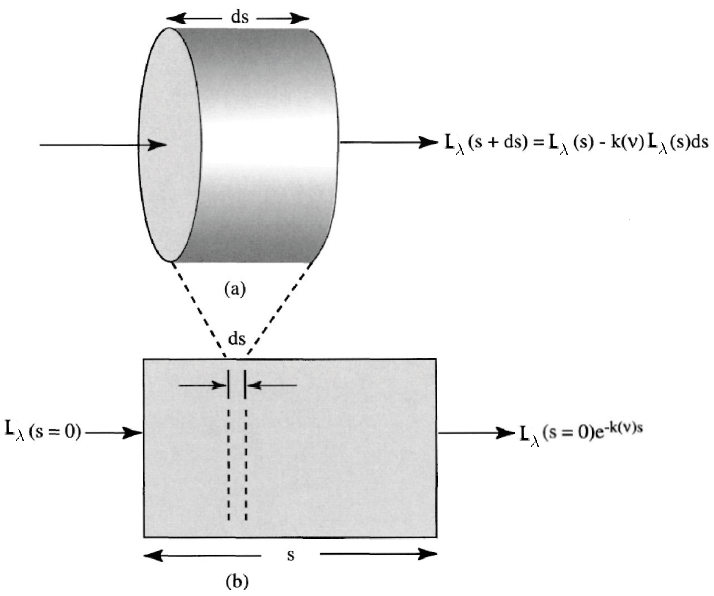
\includegraphics[width=0.6\textwidth]{sos/figures/extincion.png}
        \caption[Esquemas de extinción de la luz (Ley de Bouguer-Lambert-Beer).]{a) La radiación que pasa a través de una rodaja diferencial de materia ópticamente activa sufre una extinción proporcional al camino diferencial recorrido $ds$. b) La extinción es exponencial cuando la radiación atraviesa un camino finito $s$ dentro del material.}
        \label{sos:extincion}
        \end{figure}
        
        Se encuentra experimentalmente que el grado de decaimiento de la radiancia en un camino diferencial depende linealmente de la radiancia incidente ingresante $L(\lambda)$ y del camino $ds$ atravesado dentro del material:
        
        \begin{equation}
        dL(\lambda)\propto -L(\lambda) ds
        \label{sos:eq:laambertdif2}
        \end{equation}
        
        Dicha ecuación no es más que la versión diferencial de la ETR en que no se considera la presencia de fuentes. La constante de proporcionalidad correspondiente se denomina \textit{coeficiente de extinción del medio}, $\sigma(\lambda)$. Ahora bien, dado que se está trabajando sobre una atmósfera plano paralela, las propiedades ópticas del sistema de estudio son únicamente dependientes de la altura; por lo que es válido reemplazar:
        
        \begin{equation}
        ds=\frac{dz}{\nu}
        \label{sos:eq:z_y_s}
        \end{equation}
        
        \noindent siendo $\nu=cos(\theta)$, con lo que se obtiene la versión diferencial de la \textit{ecuación de Bouguer-Lambert-Beer} para una atmósfera plano-paralela:
        
        \begin{equation}
        \nu \frac{d L(\lambda)}{dz}=-\sigma(\lambda) L(\lambda)
        \label{sos:eq:lambertdif3}
        \end{equation}
        
        Integrando la Ec. \ref{sos:eq:lambertdif3} por separación de variables, tras considerar la Ec. \ref{sos:eq:z_y_s}, se obtiene:
        
        \begin{equation}
        L(\lambda)(z)=L(\lambda)(0)e^{-\int_{0}^{z}\frac{dz'}{\nu} \sigma(z,\lambda)}=L(\lambda)(0)e^{-\frac{\tau(z,\lambda)}{\nu}}
        \label{sos:eq:lambertint}
        \end{equation}
        
        \noindent donde se definió el \textit{espesor óptico}, $\tau(z,\lambda)$, del camino $z$, que podrá despejarse a partir de la Ec. \ref{sos:eq:lambertint}:
        
        \begin{equation}
        \tau(\lambda,z)=-ln \left( \frac{L(\lambda,z'=0)}{L(\lambda,z'=z)} \right) \quad [s/u]
        \label{sos:eq:tau_definicion}
        \end{equation}
        
        Tanto $\sigma(\lambda)$ como $\tau(\lambda)$ pueden ser divididos en sus componente debidas a la absorción (a) y a la dispersión (s):
        
        \begin{align}
         &\sigma(\lambda)=\sigma_{a}(\lambda)+\sigma_{s}(\lambda)\\
         &\tau(\lambda)=\tau_{a}(\lambda)+\tau_{s}(\lambda)
        \label{sos:eq:abs_sca}
         \end{align}
        
        Diferenciando la Ec. \ref{sos:eq:tau_definicion} respecto de $z$, se halla la siguiente relación biyectiva $\tau\leftrightarrow z$:
        
        \begin{equation}
        d\tau=\nu \frac{dL}{L}=-\sigma(z) dz
        \label{sos:eq:tau_y_z}
        \end{equation}
        
        Dicha biyección permitirá utilizar el espesor óptico medido desde el TOA hasta $z$ como variable de altura. Obsérvese que $\tau$ aumenta hacia abajo, lo que explica el signo negativo en Ec. \ref{sos:eq:tau_y_z}. El TOA corresponde a $\tau=0$ y llamaremos $\tau^{*}$ al espesor óptico en la superficie, es decir, el espesor óptico total de la atmósfera. Por lo que la Ec. \ref{sos:eq:lambertdif3} podrá ser reescrita como:
        
        \begin{equation}
        \boxed{\nu \frac{d L(\lambda)}{d\tau}=L(\lambda)}
        \label{sos:eq:LAMBERT_BEER}
        \end{equation}
        
        \noindent que será la versión de la ley de extinción sobre la cual se basará la ETR escalar.

    \subsection{La ecuación escalar de transferencia radiativa}
    \label{sos:s:EETR}
        
        La ecuación de Bouguer-Lambert-Beer tiene en cuenta la absorción y la dispersión como procesos de extinción de un haz de radiación; pero no contempla el hecho de que la luz dispersada por las partículas en la atmósfera y la proveniente de la superficie terrestre sirve también de fuente de REM en esa y otras direcciones. Para poder agregar el término de fuente a la Ec. \ref{sos:eq:LAMBERT_BEER} es necesario aún presentar dos magnitudes físicas más: la primera es el \textit{albedo de dispersión simple}, $\omega_{s}$: 
        
        \begin{equation}
         \omega_{s}=\frac{\sigma_{s}}{\sigma}
        \label{sos:eq:lenoble2}
         \end{equation}
        
        \noindent que representa la fracción de fotones que al interactuar con una partícula sufre un proceso de dispersión respecto de la totalidad de procesos considerados - es decir, absorción y dispersión.\footnote{En este apéndice se asumen como despreciables todos los eventos asociados a procesos de dispersión inelástica dada su baja incidencia en los procesos físicos estudiados en la presente tesis.}
         
        La segunda es la \textit{función de fase}, $p(\Theta)$, que describe la probabilidad de dispersión en función del ángulo $\Theta$, comprendido entre las direcciones incidente y de dispersión. $p(\Theta)$ está normalizada a $4\pi$ cuando se la integra sobre todo el ángulo sólido.
        
        Tomando la Ec. \ref{sos:eq:LAMBERT_BEER}, agregando la dependencia de las magnitudes con la dirección, y asumiendo la presencia de fuentes, se arriba a la ecuación de transferencia radiativa escalar:
        
        \begin{equation}
        \boxed{\nu \frac{d L(\lambda,\tau,\nu,\phi)}{d\tau}=L(\lambda,\tau,\nu,\phi)+S(\lambda,\tau,\nu,\phi)}
        \label{sos:eq:EETR}
        \end{equation}
        
        \noindent donde $S(\lambda,\tau,\nu,\phi)$ es la \textit{función fuente}, y la misma viene dada por:
        
        \begin{equation}
        \begin{split}
        S(\lambda,\tau,\nu,\phi) =&\frac{\omega_{s}(\tau)}{4 \pi} 
        p(\lambda,\tau,\nu,\phi,cos(\theta_{s}),\phi_{s}) E_{s} e^{-\frac{\tau}{cos(\theta_{s})}} 
        +\\ &\frac{\omega_{s}(\tau)}{4 \pi} \int_{0}^{2\pi} 
        \int_{-1}^{1} p(\lambda,\tau,\nu,\phi,\nu',\phi') L(\lambda,\tau,\nu',\phi')d\nu'd\phi'
        \end{split}
        \label{sos:eq:fuente_escalar}
        \end{equation}
        
        \noindent donde se han incluido el término asociado a la luz solar directa (términos con subíndice \textit{s}) y el asociado a radiación proveniente de procesos de dispersión.
        
    \subsection{Los parámetros de Stokes}
    \label{sos:s:stokes}
        
        Dado que los procesos de dispersión dependen del estado de polarización, y la modifican, la radiancia derivada a partir de la ecuación escalar (Ec. \ref{sos:eq:EETR}) es una aproximación que puede diferir del valor exacto hasta en un $10$ \%. Es por esto que se utilizarán los parámetros de Stokes, que contienen información del estado de polarización de la radiación.
        
        Una onda electromagnética viajando en la dirección $\bf{k}$ es caracterizada por las componentes complejas $E_{l}$ y $E_{r}$ del campo eléctrico $\bf{E}$, correspondientes a las proyecciones en los versores ortogonales $\bf{l}$ y $\bf{r}$ contenidos en el frente de ondas (de forma tal de que $(\bf{l},\bf{r},\bf{k})$ conforma una terna derecha), o por cualquier combinación de los cuatro parámetros $E_{l}\hat{E}_{l}$, $E_{r}\hat{E}_{r}$, $E_{r}\hat{E}_{l}$ y $E_{l}\hat{E}_{r}$, donde $\hat{E}$ representa el valor conjugado de $E$. Los parámetros de Stokes quedan definidos por
        
        \begin{equation}
        \begin{bmatrix} 
        I \\ Q \\ U \\ V 
        \end{bmatrix}
        =\frac{\epsilon_{0}c}{2}
        \begin{bmatrix}
        \left<{E_{l}\hat{E}_{l}}\right>+\left<{E_{r}\hat{E}_{r}}\right>\\
        \left<{E_{l}\hat{E}_{l}}\right>-\left<{E_{r}\hat{E}_{r}}\right> \\
        \left<{E_{l}\hat{E}_{r}}\right>+\left<{E_{r}\hat{E}_{l}}\right> \\
        i\left<{E_{l}\hat{E}_{r}}\right>-i\left<{E_{r}\hat{E}_{l}}\right> 
        \end{bmatrix}
        =\frac{\epsilon_{0}c}{2}
        \begin{bmatrix}
        \left<{E_{l0}^{2}}\right>+\left<{E_{r0}^{2}}\right>\\
        \left<{E_{l0}^{2}}\right>-\left<{E_{r0}^{2}}\right>\\
        2\left<{E_{l0}E_{r0}cos(\delta)}\right>\\
        2\left<{E_{l0}E_{r0}sin(\delta)}\right>
        \end{bmatrix}
        \label{sos:eq:lenoble5}
        \end{equation}
        
        \noindent donde $E_{l0}$ y $E_{r0}$ son las amplitudes de $E_{l}$ y $E_{r}$, respectivamente, y $\delta$ es la fase de retardación de $E_{l}$ respecto de $E_{r}$; $c$ es la velocidad de la luz y $\epsilon_{0}$ la constante dieléctrica en el vacío, respectivamente. Dado que las mediciones siempre incluyen grandes números de trenes de ondas, las cantidades $\left<{x}\right>$ son los promedios temporales de $x$ (en caso de ser ondas monocromáticas, vale, en este contexto, que $\left<{x}\right>=x$). Los parámetros de Stokes contienen toda la información del campo de radiación. $I$ es la energía total de radiación, es decir, equivalente a la irradiancia $E$, o la radiancia $L$, consideradas en la sección anterior. Los otros tres parámetros tienen las mismas dimensiones que $I$ ($W/m^{-2}$ o $W/m^{-2}sr^{-1}$, según la ocasión); sirven para caracterizar el estado de polarización. El mismo es determinado por $\delta$ y por la razón $a=\frac{E_{l0}}{E_{r0}}$. Para una mezcla de trenes de onda incoherentes, con las mismas amplitudes promedio, $Q=U=V=0$, entonces la radiación es natural o no polarizada. Este es el caso de la radiación solar extraatmosférica (Figura \ref{int:hiper_thuillier}). Dada la aditividad de los parámetros de Stokes, cualquier haz puede ser analizado como la superposición incoherente de radiación polarizada con una intensidad

        \begin{equation}
         I_{pol}=(Q^{2}+U^{2}+V^{2})^{1/2}
        \label{sos:eq:lenoble6}
         \end{equation}

        \noindent y radiación natural; siendo el grado de polarización:
        
        \begin{equation}
        P=I_{pol}/I
        \label{sos:eq:lenoble7}
        \end{equation}

        Para polarización lineal, $\delta=0$ y $V=0$, y $Q$ y $U$ fijan la dirección de polarización. Si $\alpha$ es el ángulo de rotación alrededor de $\bf{k}$ que alínea $\bf{l}$ a $\bf{E}$, se tienen
        
        \begin{equation}
        Q=I_{pol}cos(2\alpha)\quad
        U=I_{pol}sin(2\alpha)
        \label{sos:eq:lenoble8}
        \end{equation}

        Para luz elípticamente polarizada, el parámetro $V$ define la elipticidad de la luz polarizada; $V$ es generalmente muy chico en la atmósfera y es usualmente despreciado, por lo que el estado de polarización puede ser considerado lineal. La radiancia (irradiancia), cantidad usualmente escalar, será convenientemente reemplazada por el vector radiancia (irradiancia), construido a partir de los parámetros de Stokes:
        
        \begin{equation}
         \bf{L}=(I,Q,U,V)^{T}
        \label{sos:eq:lenoble9}
         \end{equation}

        \noindent donde $\bf{x}^{T}$ representa el transpuesto del vector $x$.

    \subsection{La matriz de fase}
    \label{sos:s:matrizdefase}

        Para poder describir el fenómeno de dispersión considerando el estado de polarización, se deberá reemplazar la función de fase escalar, $p(\Theta)$, por una matriz de $4 \times 4$. Se elegirán los ejes de referencia $(\bf{l'},\bf{r'})$ y $(\bf{l},\bf{r})$, para la radiación incidente y dispersada en dirección paralela ($\bf{l}$) y perpendicular ($\bf{r}$) al plano de dispersión, definido por las direcciones de incidencia y dispersión. Para una distribución de partículas orientadas al azar, en igual cantidad que sus respectivos quirales (partículas espejadas), condición no muy restrictiva para los aerosoles, la matriz de fase queda, a partir de la teoría de Mie, \cite{mishchenko2002}, en la forma:
        
        \begin{equation}
        \bf{P}(\Theta)=
        \begin{bmatrix}
        {P_{11}(\Theta)}&{P_{12}(\Theta)}&{0}&{0} \\
        {P_{21}(\Theta)}&{P_{22}(\Theta)}&{0}&{0} \\
        {0}&{0}&{P_{33}(\Theta)}&{P_{34}(\Theta)}\\
        {0}&{0}&{P_{43}(\Theta)}&{P_{44}(\Theta)}\\
        \end{bmatrix}
        \label{sos:eq:lenoble10}
        \end{equation}
        
        \noindent donde $P_{21}=P_{12}$ y $P_{43}=-P_{34}$, y el elemento $P_{11}(\Theta)$ es idéntico a la función de fase $p(\Theta)$. A su vez, para partículas esféricas (asunción que se hará sobre los aerosoles) se tiene que $P_{22}=P_{11}$ y $P_{44}=P_{33}$. Para moléculas anisótropas (caso de la dispersión por Rayleigh) vale que $P_{34}=P_{43}=0$; pero $P_{44}\neq P_{33}$ y $P_{44}\neq P_{33}$.


    \subsection{La ecuación vectorial de transferencia radiativa}
    \label{sos:s:EVTR}
    
        La transferencia radiativa dentro de la atmósfera es gobernada por la ecuación homónima, cuya versión escalar (EETR) se expresa en Ec. \ref{sos:eq:EETR}. Ahora, como bien se comentó previamente, es necesario incluir efectos de polarización. Dado que los parámetros de Stokes son aditivos ante la superposición de rayos, una ecuación vectorial que gobierne al vector $L(\lambda,\theta,\nu,\phi)$ puede ser establecida de la misma manera que el caso de la ecuación escalar. La condición es que todos los parámetros de Stokes sumados estén referidos a las mismas direcciones \textbf{l} y \textbf{r}; la elección más obvia es tomar \textbf{l} y \textbf{r} paralelo y perpendicular al plano vertical conteniendo a \textbf{k}. Cuando la radiación incidente de la dirección $(\nu',\phi')$ es dispersada hacia la dirección $(\nu,\phi)$ es necesario realizar una doble rotación; dado que la matriz de dispersión está definida con ejes paralelo y perpendicular al plano de dispersión. Primero, los ejes $(\textbf{l}',\textbf{r}')$  asociados a la radiación incidente son rotados alrededor de $\textbf{k}'$ en un ángulo $\chi'$ para traerlos paralelo y perpendicular al plano de dispersión. Tomando $\chi'$ como positivo en sentido antihorario alrededor de $\textbf{k}'$, esta rotación corresponde a multiplicar la matriz de radiación por la matriz de transformación

        \begin{equation}
         \textbf{T}(\chi')=
         \begin{bmatrix}
        {1} & {0} & {0} & {0}\\
        {0} & {cos(2\chi')} & {sin(2\chi')} & {0}\\
        {0} & {-sin(2\chi')} & {cos(2\chi')} & {0}\\
        {0} & {0} & {0} & {1}\\
          \end{bmatrix}
        \label{sos:eq:lenoble15}
        \end{equation}

        Luego de aplicar la matriz de fase $\textbf{P}(\Theta)$ para el ángulo $\Theta$ entre las direcciones $(\nu',\phi')$ y $(\nu,\phi)$, una segunda rotación en $-\chi$ es realizada, con el fin de tener la matriz de radiancia dispersada referida a $(\textbf{l},\textbf{r})$
        
        Por analogía con la Ec. \ref{sos:eq:EETR}, se tiene entonces la ecuación vectorial de transferencia radiativa (EVTR):

        \begin{equation}
        \nu \frac{d \bf{L}(\lambda,\tau,\nu,\phi)}{d 
        \tau}=\bf{L}(\lambda,\tau,\nu,\phi)+\bf{S}(\lambda,\tau,\nu,\phi)
        \label{sos:eq:lenoble16a}
        \end{equation}
        
        \noindent con $\bf{S}$ la función fuente, que ahora toma la forma:
        
        \begin{align}
        \begin{split}
        \textbf{S}(\lambda,\tau,\nu,\phi) =&\frac{\omega_{s}(\tau)}{4 \pi} 
        \textbf{P'}(\lambda,\tau,\nu,\phi,\nu_{0},\phi_{0})  \bf{E}_{0} e^{\frac{\tau}{\nu_0}} 
        +\\ &\frac{\omega_{s}(\tau)}{4 \pi} \int_{0}^{2\pi} 
        \int_{-1}^{1} \textbf{P'}(\lambda,\tau,\nu,\phi,\nu',\phi') \bf{L}(\lambda,\tau,\nu',\phi')d\nu'd\phi'
        \label{sos:eq:lenoble16b}
        \end{split}
        \end{align}
        
        El primer término corresponde a la dispersión simple del haz solar directo, y el segundo a eventos de dispersión múltiple, de manera equivalente a la Ec. \ref{sos:eq:fuente_escalar}. Aquí, $\bf{P'}$ corresponde a la matriz de fase rotada según lo expuesto en la Ec. \ref{sos:eq:lenoble15}. Como fue dicho previamente, no se considerará la emisión térmica proveniente de la función fuente. La matriz $\textbf{P}$ de $4 \times 4$ en Ec. \ref{sos:eq:lenoble16b} es
        
        \begin{equation}
         \textbf{P}(\lambda,\tau,\nu,\phi,\nu',\phi')=\textbf{T}(-\chi)\textbf{P}(\tau,\Theta)\textbf{T}(\chi')
        \label{sos:eq:lenoble17}
         \end{equation}
        
        \noindent y el vector de irradiancia para la radiación solar incidente (no polarizada) es
        
        \begin{equation}
        \textbf{E}_{0}=(E_{0},0,0,0)^{T}
        \label{sos:eq:lenoble18}
        \end{equation}
        
        Integrando la Ec. \ref{sos:eq:lenoble16a} obtenemos
        
        \begin{equation}
        \textbf{L}(\lambda,\tau,\nu<0,\phi) = 
        -\int_{0}^{\tau}e^{-\frac{\tau'-\tau}{\nu}}\textbf{S}(\lambda,\tau', 
        \nu,\phi)d\tau'/\nu
        \label{sos:eq:lenoble19a}
        \end{equation}
        
        \begin{equation}
        \textbf{L}(\lambda,\tau,\nu>0,\phi)= 
        \textbf{L}^{up}(\tau^{*},\nu>0,\phi)e^{-\frac{\tau^{*}-\tau}{\nu}}+\int_{\tau}^{\tau^
        {*}}e^{-\frac{\tau'-\tau}{\nu}}\textbf{S}(\lambda,\tau', \nu, \phi)d\tau'/\nu
        \label{sos:eq:lenoble19b}
        \end{equation}
        
        En el caso en que se desprecie la radiación difusa incidente a TOA, $\textbf{L}^{up}$ depende de la reflectancia superficial, que es nula para una superficie negra. Las ecuaciones \ref{sos:eq:lenoble19a} y \ref{sos:eq:lenoble19b} son la forma de la EVTR expresadas en la forma con la que el método de órdenes sucesivos de dispersión trabaja. La EVTR es equivalente a cuatro ecuaciones acopladas para los parámetros de Stokes $I$, $Q$, $U$ y $V$ que conforman la radiancia vectorial $\textbf{L}$. La EETR es simplemente la primera de estas ecuaciones  escrita para $L=I$, con $Q=U=V=0$, y $P_{11}=p$, la función de fase, teniendo en cuenta que $\textbf{T}$ no afecta esta primera componente.

\section{El código de órdenes sucesivos de dispersión (SOS)}
\label{sos:s:sos}
    El código de transferencia radiativa utilizado en la presente tesis se denomina de Órdenes Sucesivos de Dispersión (\textit{Successive Orders of Scattering}, SOS) y fue implementado por primera vez por M. Deuzé en 1974, \cite{lafrance2002}, en el \textit{Laboratoire d' Optique Atmosphérique} en Francia. Desde entonces hasta su versión actual, 5.0, el mismo ha sufrido sucesivas readaptaciones para enfocarlo en el estudio del sistema Tierra-Atmósfera. El código SOS computa la transferencia radiativa vectorial y utiliza el método de Órdenes Sucesivos de Dispersión, con la importante propiedad de estar orientado al estudio de procesos en los que la dispersión domine por sobre la emisión térmica, que es el caso de interés. El mismo cuenta con la posibilidad de modelar sistemas con superficies tanto terrestres como marinas, cuyas propiedades ópticas pueden ser reguladas a partir de parámetros ópticos propuestos por un conjunto amplio de modelos. Entre estos, se halla por ejemplo, el modelo de \textit{sunglint} de Cox y Munk, \cite{coxmunk1954}, para superficies marinas con rugosidad debida al viento en superficie (véase Figura \ref{int:s:sunglint}).
    
    El mismo es utilizado para simular las radiancias a TOA y resuelve la Ec. \ref{sos:eq:lenoble16a} a partir del \textit{método SOS} y separando en series de Fourier la dependencia acimutal de las magnitudes calculadas.

    \subsection{El método de órdenes sucesivos de dispersión}
    \label{sos:s:metodosos}

        La idea subyacente al método de órdenes sucesivos de dispersión es separar la radiancia en las contribuciones de los fotones dispersados una, dos, ..., $n$ veces.
        
        \begin{equation}
        \textbf{L}(\lambda,\tau,\nu,\phi)=\sum_{n=1}^{N}\textbf{L}_{n}(\lambda,\tau,\nu,\phi)
        \label{soslenoble20}
        \end{equation}
        
        Esto fue sugerido por primera vez por Hammad y Chapman, \cite{hammad1948}; aunque estos utilizaban únicamente los primeros dos términos, y luego utilizado por varios autores en diversas variantes, y recientemente por Min y Duan \cite{min2004}. Partiendo de las Ecs. \ref{sos:eq:lenoble19a} y \ref{sos:eq:lenoble19b}, esto lleva a:
        
        \begin{equation}
        \textbf{L}_{n}(\lambda,\tau,\nu<0,\phi) = 
        -\int_{0}^{\tau}e^{-\frac{\tau'-\tau}{\nu}}\textbf{S}_{n}(\lambda,\tau', 
        \nu,\phi)d\tau'/\nu
        \label{lenoble21a}
        \end{equation}
        
        \begin{equation}
        \textbf{L}_{n}(\lambda,\tau,\nu>0,\phi)= 
        \textbf{L}_{n}^{up}(\lambda,\tau^{*},\nu>0,\phi)e^{-\frac{\tau^{*}-\tau}{\nu}}+\int_{\tau}^{\tau^
        {*}}e^{-\frac{\tau'-\tau}{\nu}}\textbf{S}_{n}(\lambda,\tau', \nu, \phi)d\tau'/\nu
        \label{lenoble21b}
        \end{equation}
        
        \noindent donde $\tau^{*}$ corresponde al espesor óptico total de la atmósfera y los diferentes órdenes de la función fuente están dados a su vez  por:
        
        \begin{equation}
        \textbf{S}_{1}(\lambda,\tau,\nu,\phi) = \frac{\omega_{s}(\tau)}{4 \pi} 
        \textbf{P}(\lambda,\tau,\nu,\phi,\nu_{0},\phi_{0})  \textbf{E}_{0} e^{-\frac{\tau}{\nu_0}} 
        \label{sos:eq:lenoble21c}
        \end{equation}
        
        
        \begin{equation}
        \textbf{S}_{n>1}(\lambda,\tau,\nu,\phi)= \frac{\omega_{s}(\tau)}{4 \pi} \int_{0}^{2\pi} 
        \int_{-1}^{1} \textbf{P}(\lambda,\tau,\nu,\phi,\nu',\phi') \textbf{L}_{n-1}(\lambda,\tau,\nu',\phi')d\nu'd\phi',
        \label{sos:eq:lenoble21d}
        \end{equation}
        
        \noindent y considerando que una reflexión es semejante a un proceso de dispersión:
        
        
        \begin{equation}
        \textbf{L}_{1}^{up}(\lambda,\tau^{*},\nu>0,\phi) = -\frac{cos(\theta_{s})}{\pi} 
        \textbf{R}(\lambda,\nu,\phi,cos(\theta_{s}),\phi_{s}) \textbf{E}_{s}  e^{\frac{\tau^{*}}{cos(\theta_{s})}} 
        \label{sos:eq:lenoble21e}
        \end{equation}
        \begin{equation}
        \textbf{L}_{n>1}^{up}(\lambda,\tau^{*},\nu<0,\phi)= \int_{0}^{2\pi} \int_{-1}^{0} 
        (-\frac{\nu'}{\pi}) R(\lambda,\nu,\phi,\nu',\phi') 
        \textbf{L}_{n-1}(\lambda,\tau^{*},\nu',\phi')d\nu'd\phi'
        \label{sos:eq:lenoble21f}
        \end{equation}
        
        La Ec. \ref{sos:eq:lenoble21e} define la matriz de reflectancia de la superficie, $\textbf{R}(\lambda,\nu,\phi,cos(\theta_{s}),\phi_{s})$, como una generalización de la reflectancia escalar del caso lambertiano.
        
    \subsection{Expansión en series de Fourier de la dependencia acimutal}
    \label{sos:s:fourierAcimutal}

        Las dependencias acimutales son separadas y expandidas por el código en series de  Fourier, por ej. para $\textbf{L}_{n}$, Ec. \ref{sos:eq:lenoble21f}, se tiene:
        
        \begin{equation}
        \textbf{L}_{n}(\tau,\nu,\phi)=\sum_{s=0}^{S}(2-\delta_{0s})cos(s(\phi-\phi_{0}))\textbf{L}_{n}^{s}
        (\tau,\nu)
        \label{sos:eq:SOS_FOURIER}
        \end{equation}
        
        \noindent donde \textit{S} es un parámetro de corte, especificado - y modificable - dentro del código. Tanto los órdenes sucesivos de dispersión como los de Fourier aportan cantidades cada vez menores al aumentar los órdenes $n$ y $s$,  respectivamente, por lo cual, el código implementa dos tests de convergencia, uno por cada índice en cuestión, que truncan sendos desarrollos a partir de que los términos sucesivos se tornan insignificantes \cite{lafrance2002}.